\section{Implementation and Evaluation} \label{sec:sec4}

\subsection{Data description and Pre-processing}

We built our experiment based on networkx-1.10\footnote{\url{http://networkx.github.io/}}, a well-known Python language software package for the creation, manipulation, and study of the structure, dynamics, and functions of complex networks. During the experiment, we applied random partition algorithm (a naive implementation), community detection (provided by community module\footnote{\url{http://perso.crans.org/aynaud/communities/}}) and metis partition (provided by nxmetis module\footnote{\url{http://networkx-metis.readthedocs.org/en/latest/}}). We ran our experiment on a Ubuntu 15.04 workstation with 16G RAM and an Intel Xeon 12-core processor. The Python version is 2.7.9. Our implementation code and the resultant data is available at GitHub\footnote{\url{https://github.com/HongxuChen/ds_assign1}}. 

The input data is collected from the SNAP page\footnote{\url{https://snap.stanford.edu/data/}} provided by J. McAuley and J. Leskovec.~\cite{Mcauley:2014:DSC:2582178.2556612}. We selected 3 datasets: Facebook, DBLP, and YouTube. All of our chosen raw graph data is represented as lines of edge pairs in a gzip file. In order to load the data fast, we did a pre-processing work that pickled each graph object in a data stream file.

We provided an elementary analysis (\textsf{graph\_info.py}) on the graphs to get an overview of these data, including the node size, edge size, average clustering coefficient, number of triangles, etc. The results are shown in Table \ref{tbl:graphinfo} and can be confirmed in their SNAP pages.

Additionally, we pre-computed the node degree list and sorted them in a descending order $D=\langle nd_1, nd_2, \ldots, nd_n\rangle$, where each element $nd_i, i\in \left\{1,2,\ldots, n\right\}$ is a pair $(n_i, d_i)$ which represents the node and its degree respectively.


\begin{table}[]
\centering
\caption{Basic Graph Information}
\label{tbl:graphinfo}
\begin{tabular}{|c|c|c|c|c|c|}
\hline
\textbf{} & \textbf{\# node} & \textbf{\# edge} & \textbf{clustering} & \textbf{\# triangles} & \textbf{type} \\ \hline
\textbf{Facebook} & 4039 & 88234 & 0.6055 & 1612010 & social \\ \hline
\textbf{DBLP} & 317080 & 1049866 & 0.6324 & 2224385 & \begin{tabular}[c]{@{}c@{}}ground-truth\\ communities\end{tabular} \\ \hline
\textbf{YouTube} & 1134890 & 2987624 & 0.0808 & 3056386 & \begin{tabular}[c]{@{}c@{}}ground-truth\\ communities\end{tabular} \\ \hline
\end{tabular}
\end{table}

\subsection{Comparison of Partitioning Algorithms} \label{sec:exp1}

This experiment compares the locality for different partition strategies without replication or temporary caching. 

Our experiments are conducted with such an assumption: all nodes in the graph are accessed with equal opportunities, and accessing each node requires to retrieve \emph{all} of the neighbor nodes $neighbor(n)$. 

As we do not consider the data replication when a node data is stored remotely and do not care about the data fetch mechanism (e.g., caching frequently accessed data), the locality problem is only relevant to the static node distribution against a particular partitioning approach. A generated partitioning divides the underlying node set $N$ into $m$ parts: $\mathcal{N}=\left\{N_1, N_2, \ldots , N_m\right\}$. For each $n\in N_i, i\in \left\{1,2,\ldots, m\right\}$, we compute the number of its neighbor nodes that are also in $N_i$, i.e., 

\begin{equation*}
	Local(n) = |neighbor(n) \cap N_i|, n\in N_i
\end{equation*}

And the graph locality is measured as the ratio of summation of node localities against the summation of all nodes' degrees.

\begin{equation*}\label{eq:locality}
	\mathcal{L}(G) = \frac{\Sigma _{n\in N} Local(n)}{\Sigma _{n\in N} |neighbor(n)|}
\end{equation*}

\bigskip

An interesting question is that: can we use a partial graph to approximate the result of the full graph locality information?

\bigskip

Intuitively, if we collect a node set whose element node has larger degree and get a subgraph $G'$ from the edge relationship, we may get a locality that is similar to $\mathcal{L}(G)$. To get the node set, we slice the node order list $D$ with a percentage thredshold $r\in (0,1]$, that is to say $D_r=\langle nd_1, nd_2, \ldots, nd_{\mathcal{r}}\rangle$ is a prefix of $D$ where $\mathcal{r}=r*|N|$. The node set $N_r$ consists of all nodes corresponding to the first element of $nd_i$ in each $D_r$, and $G_r$'s edge set is defined as $\left\{e\in neighbor(n)|n\in N_r\right\}$.

Since community detection algorithm partitions the graph according to the graph structure, it does not require the number of group as the input. However for METIS and random partition need that. In this sense, we use the same part number $\textsf{parts}$ as the former for the other two algorithms.


\begin{figure}[t]

  \centering
  \hfill
  \subfigure[Line Chart]{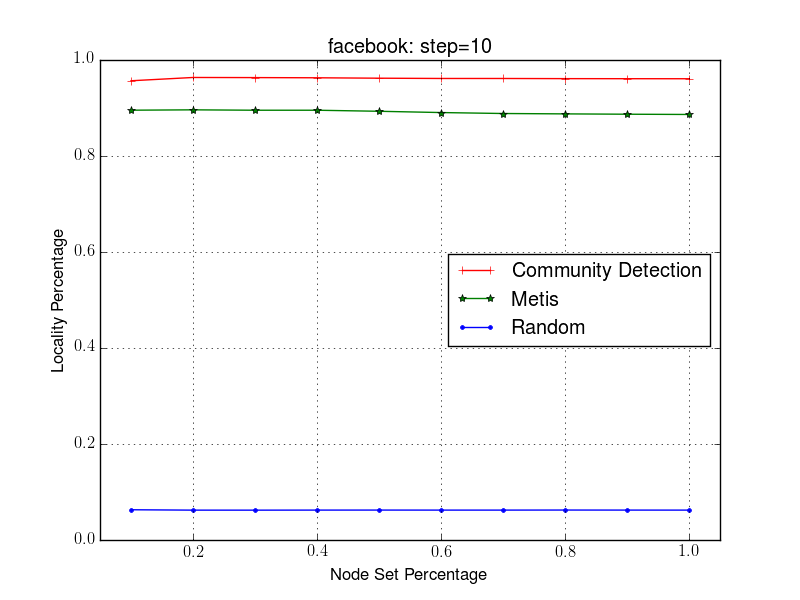
\includegraphics[width=0.45\columnwidth]{facebook_exp1.png}}
  \hfill
  \subfigure[Bar Chart]{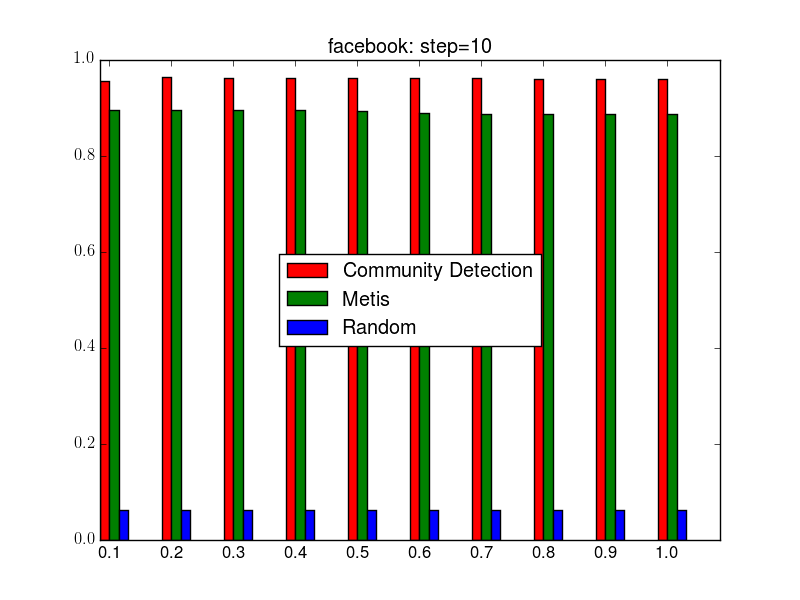
\includegraphics[width=0.45\columnwidth]{facebook_exp1_bar.png}}
  \hfill
  \caption{Partitioning Approaches in Facebook}\label{fig:exp1_facebook}
\end{figure}

\begin{figure}[t]
  \centering
  \hfill
  \subfigure[Line Chart]{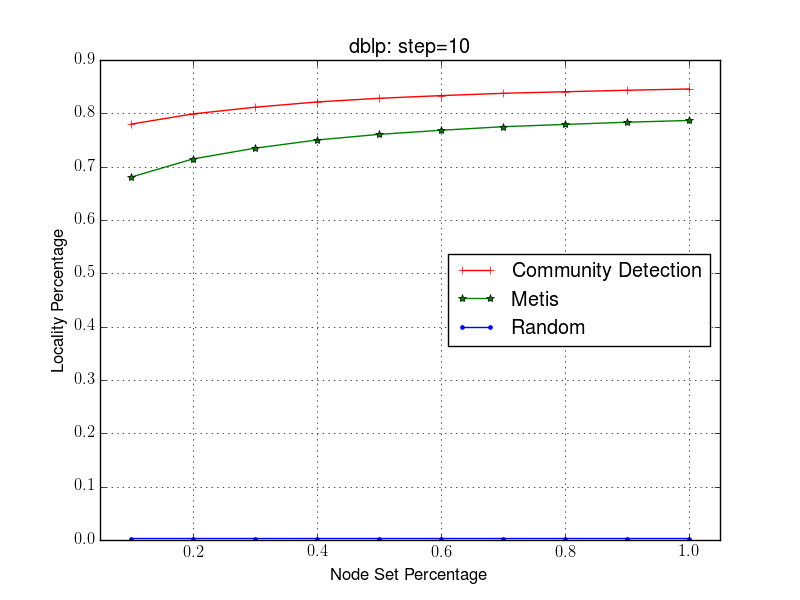
\includegraphics[width=0.45\columnwidth]{dblp_exp1.png}}
  \hfill
  \subfigure[Bar Chart]{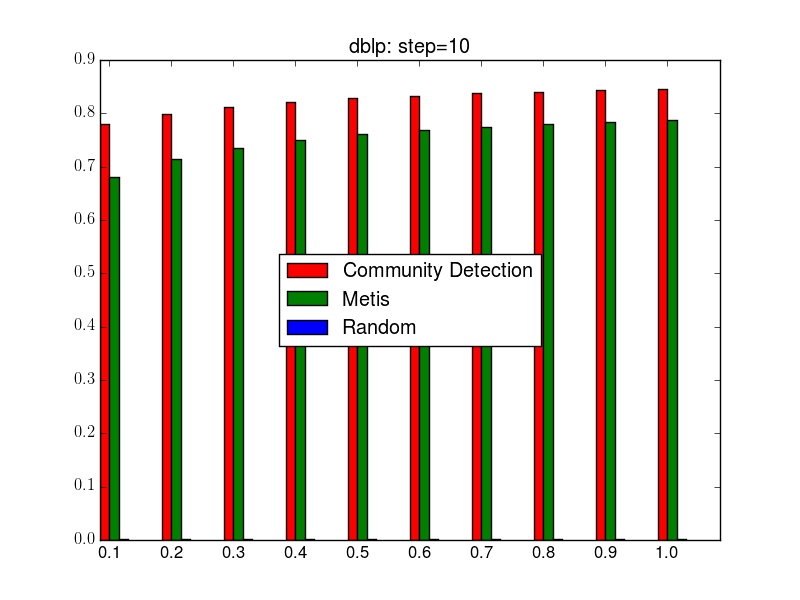
\includegraphics[width=0.45\columnwidth]{dblp_exp1_bar.png}}
  \hfill
  \caption{Partitioning Approaches in DBLP}\label{fig:exp1_dblp}
\end{figure}

\begin{figure}[t]
  \centering
  \hfill
  \subfigure[Line Chart]{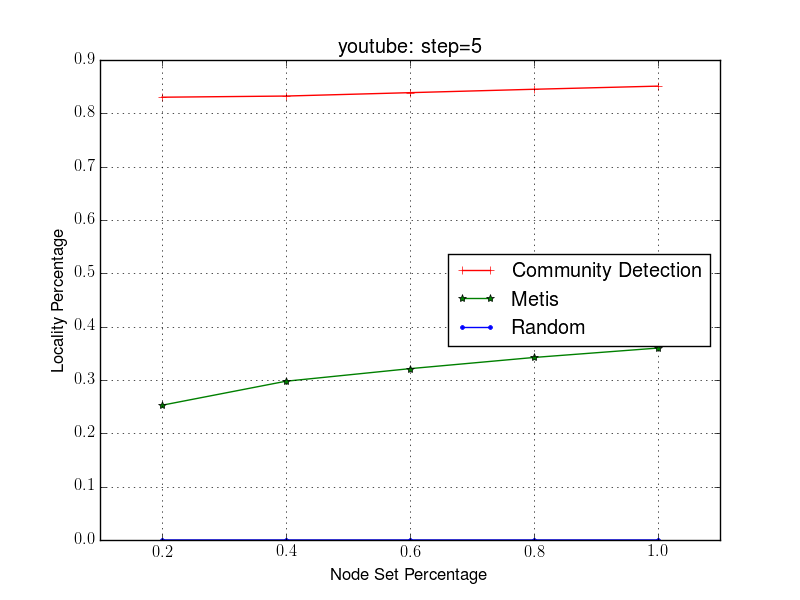
\includegraphics[width=0.45\columnwidth]{youtube_exp1.png}}
  \hfill
  \subfigure[Bar Chart]{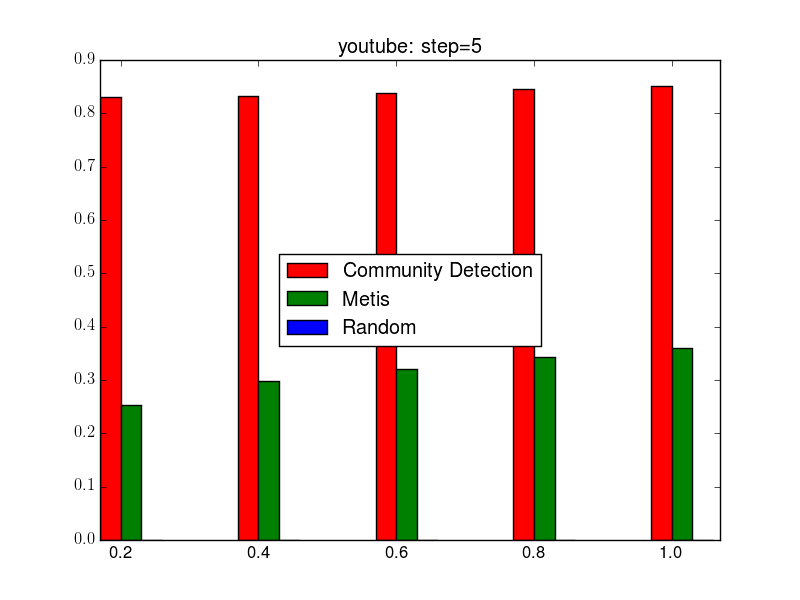
\includegraphics[width=0.45\columnwidth]{youtube_exp1_bar.png}}
  \hfill
  \caption{Partitioning Approaches in YouTube}\label{fig:exp1_youtube}
\end{figure}

Figure \ref{fig:exp1_facebook} is the result for the Facebook dataset result, we assign $r$ to be $\left\{0.1, 0.2, \ldots, 1.0\right\}$ (for YouTube it is $\left\{0.2, 0.4, \ldots, 1.0\right\}$ since otherwise it is quite costly) separately. Community Detection determines that $\textsf{parts}=16$. It is obvious that Community Detection has the largest locality and the random partition approach has the lowest average locality. Similar results also occur for DBLP \ref{fig:exp1_dblp} and YouTube \ref{fig:exp1_youtube}. By comprising Figure \ref{fig:exp1_facebook}, \ref{fig:exp1_dblp} and \ref{fig:exp1_youtube}, we can also discover that on a larger network such as the YouTube data, the locality of local clustering based algorithm METIS decreases heavily.

It is also interesting to notice that those nodes that have more neighbors have a greater impact on the locality: $\mathcal{L}(G_r)$ can somewhat represent the whole graph locality $\mathcal{L}(G)$ ($r=1.0$).

\subsection{Impact of Partition Number} \label{sec:exp2}

It is widely accepted that partition is important for distributed networks. Surely, with more data distributed in different network nodes, data will be more likely to be stored remotely. However it remains an open question how partition number affects the locality in the absence of replication.

This experiment demonstrates that how the partition number \textsf{parts} affects the locality, without considering the workload of each network node (i.e., the partition group). We only use METIS and random partition in our experiment. We range \textsf{parts} in $\left\{2, 3, \ldots, 16\right\}$ (for YouTube it is $\left\{2, 3, \ldots, 16\right\}$) and experiment on each graph.

As to the locality measurement, we use a similar way in Section \ref{sec:exp1} to compute different $G_r$ (where $r$ is set to be 0.2, 0.4, 0.6, 0.8, 1.0 separately). The final Locality $\mathcal{L}$ is computed as the average of the computed values.

The result is depicted in Figure \ref{fig:exp2}. It can be seen that the locality is decreased with the increase of partition groups. However the decrease of METIS is much slower than the random partition (for Facebook, DBLP and YouTube the lowest locality is still above $80\%$.

From the curve shown in Figure \ref{fig:exp2} and the results in Section \ref{sec:exp1}, we may conjecture that the random partition approach is too coarse that the locality coefficient $\mathcal{L}$ is in proportion to $1/\textsf{parts}$. In order to prove that, we redraw the plot where the $y-$axis to be the value of $\textsf{parts}*\mathcal{L}$ (Figure \ref{fig:rnd}).

We found that the $y-$axis value of the newly generated curve is around $1.0$ for our dataset. This convinced us that that the locality of random partition approach should suffer much since the value is in inverse proportion to the partition number \textsf{parts}.

\begin{figure}[t]
  \hfill
  \subfigure[Facebook]{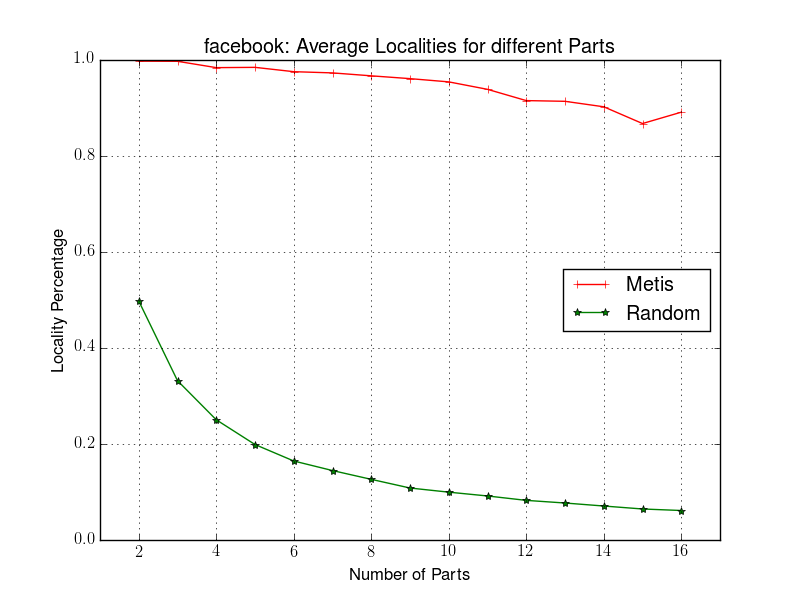
\includegraphics[width=0.45\columnwidth]{facebook_exp2.png}}
  \hfill
  \subfigure[DBLP]{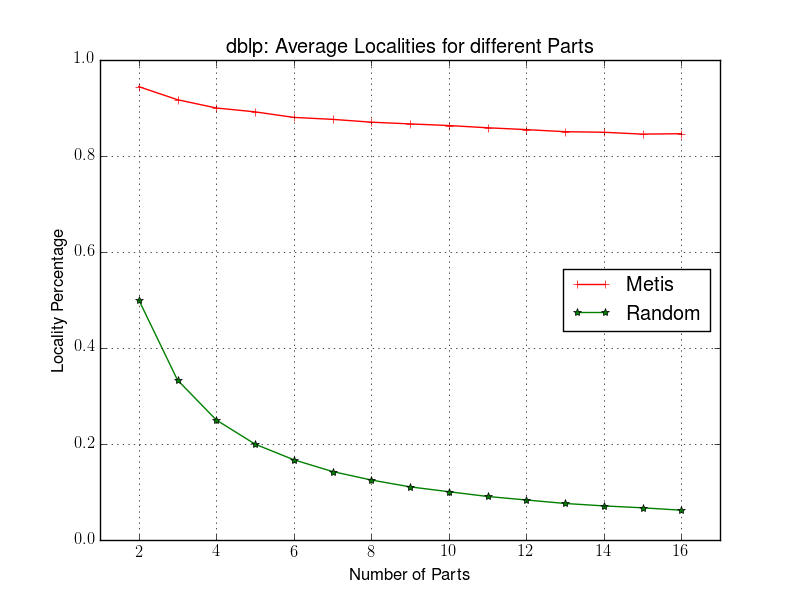
\includegraphics[width=0.45\columnwidth]{dblp_exp2.png}}
  \hfill
  \centering
  \subfigure[YouTube]{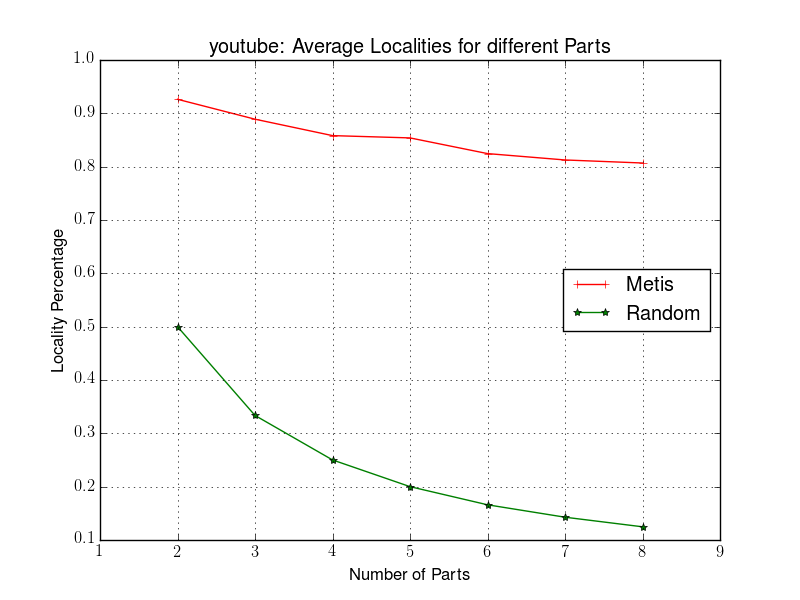
\includegraphics[width=0.45\columnwidth]{youtube_exp2.png}}
  \caption{Partition Number's Effect on Locality}\label{fig:exp2}
\end{figure}

\begin{figure}[t]
\label{fig:rnd}
  \hfill
  \subfigure[Facebook]{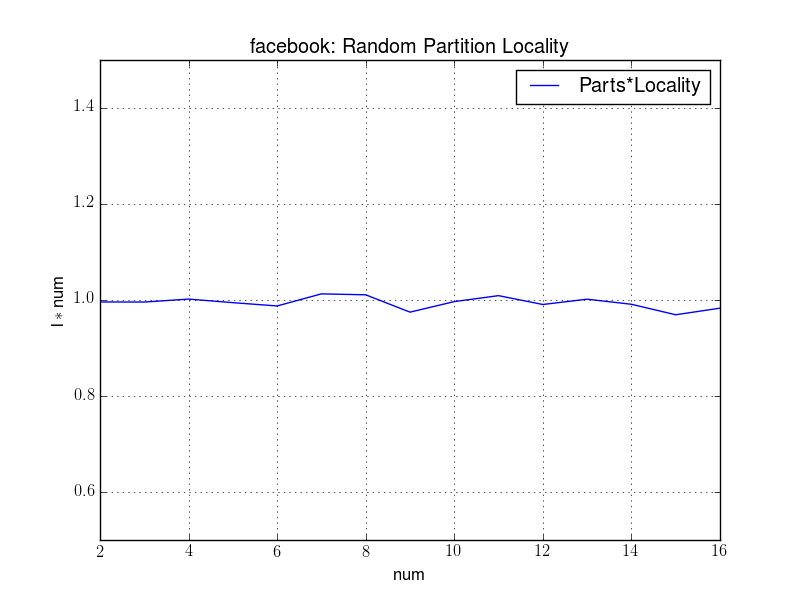
\includegraphics[width=0.45\columnwidth]{facebook_exp2_rnd.png}}
  \hfill
  \subfigure[DBLP]{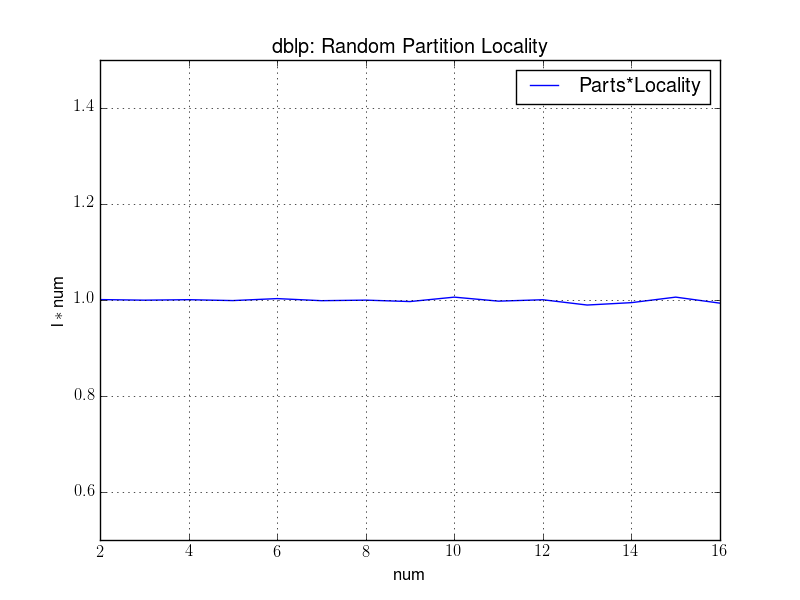
\includegraphics[width=0.45\columnwidth]{dblp_exp2_rnd.png}}
  \centering
    \subfigure[YouTube]{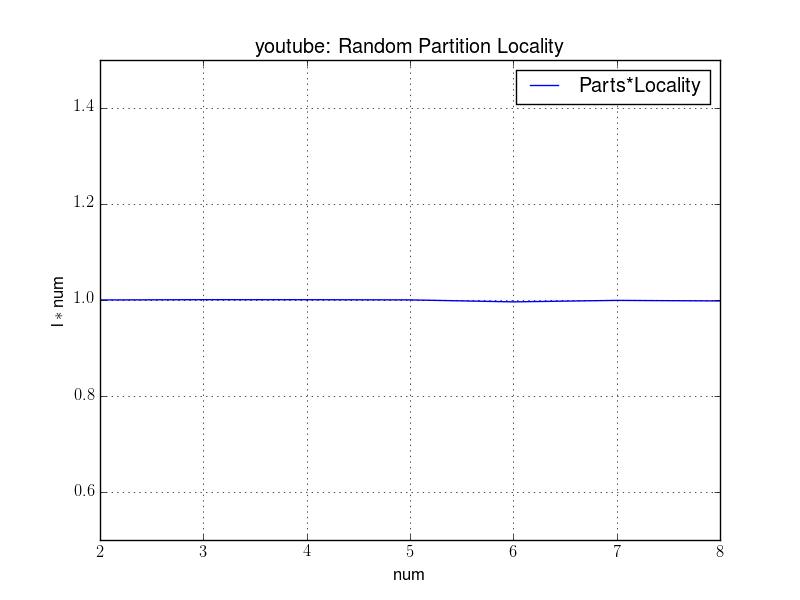
\includegraphics[width=0.45\columnwidth]{youtube_exp2_rnd.png}}
  
  \caption{Random Partitions and Localities}\label{fig:rnd}
\end{figure}

\subsection{Discussions}
It is no wonder that community detection preserves the largest locality among the three applied algorithms since community detection exhaustively computes the connection gain throughout the full graph. Meanwhile, METIS also shows a relatively high locality. The time cost for community detection can be a big issue as the graph complexity increases. For example, it takes $1.46$s for Facebook, while for DBLP and YouTube, the cost is $70.14$s and $180.74$s. This indicates that community detection may be overkill to be applied for a static network. In our experiment, METIS leverages the locality and the time cost well.

It is worth noting that in reality the network may update frequently; this is especially true for social networks such as Facebook and Twitter. This means that partition algorithms such as community detection, METIS should be recomputed each time and the existing node should be rearranged. Therefore, random partitioning may still have the advantage to be widely used; in our experiment, even for YouTube, the partitioning is finished within $0.58$s.